% Fundamental packages
\documentclass[11pt,a4paper,twoside]{book}
\usepackage[utf8]{inputenc}
\usepackage[american]{babel}
\usepackage{amsmath}
\usepackage{amsfonts}
\usepackage{amssymb}
\usepackage{graphicx}

% margins and general lay-out
%\usepackage[inner=3cm,outer=2cm,top=2.5cm,bottom=2.5cm]{geometry}
\usepackage[inner=2.5cm,outer=2.5cm,top=2.5cm,bottom=2.5cm]{geometry}
\pagestyle{plain}

% fonts (Helvetica) and typographical stuff 

\usepackage[T1]{fontenc}
\usepackage{lmodern} 
\usepackage{textcomp} 
\usepackage{pifont}
\usepackage{csquotes}
\usepackage{bm}

% Setting the font should be done after loading the typographic packages which tend to 
% set a new default font. The microtype package should however be loaded after the font ...
% using san serif helvetica clone
\usepackage{helvet}
\renewcommand{\familydefault}{\sfdefault}
% phv is another posibility.
% \renewcommand\rmdefault{phv}
\usepackage{microtype}

% additional packages
\usepackage{booktabs}
\usepackage{pdfpages}
\usepackage{hyperref}
\usepackage{float}
\usepackage{todonotes}
\usepackage{caption}
\usepackage{subcaption}
\usepackage{color}

% package to manage citations
\usepackage[backend=bibtex,style=authoryear-comp,sorting=nyt,isbn=false,url=false, natbib=true]{biblatex}
\addbibresource{references.bib}

% Kill the auto-indent
\setlength\parindent{0pt}

% test package
\usepackage{lipsum}

% Packages for list of symbols and list of abbreviations
%\usepackage[nonumberlist,acronym,toc,nomain]{glossaries}
%\makeglossaries
%\input{Glossaries/Abbreviations}

% new definitions
\newcommand{\expit}{\text{expit}}

\DeclareMathOperator*{\argmax}{arg\,max}

\DeclareMathOperator*{\argmin}{arg\,min}

% start of the document
\begin{document}

% include cover page + copyright statement + no pagenumbers
\pagenumbering{gobble}
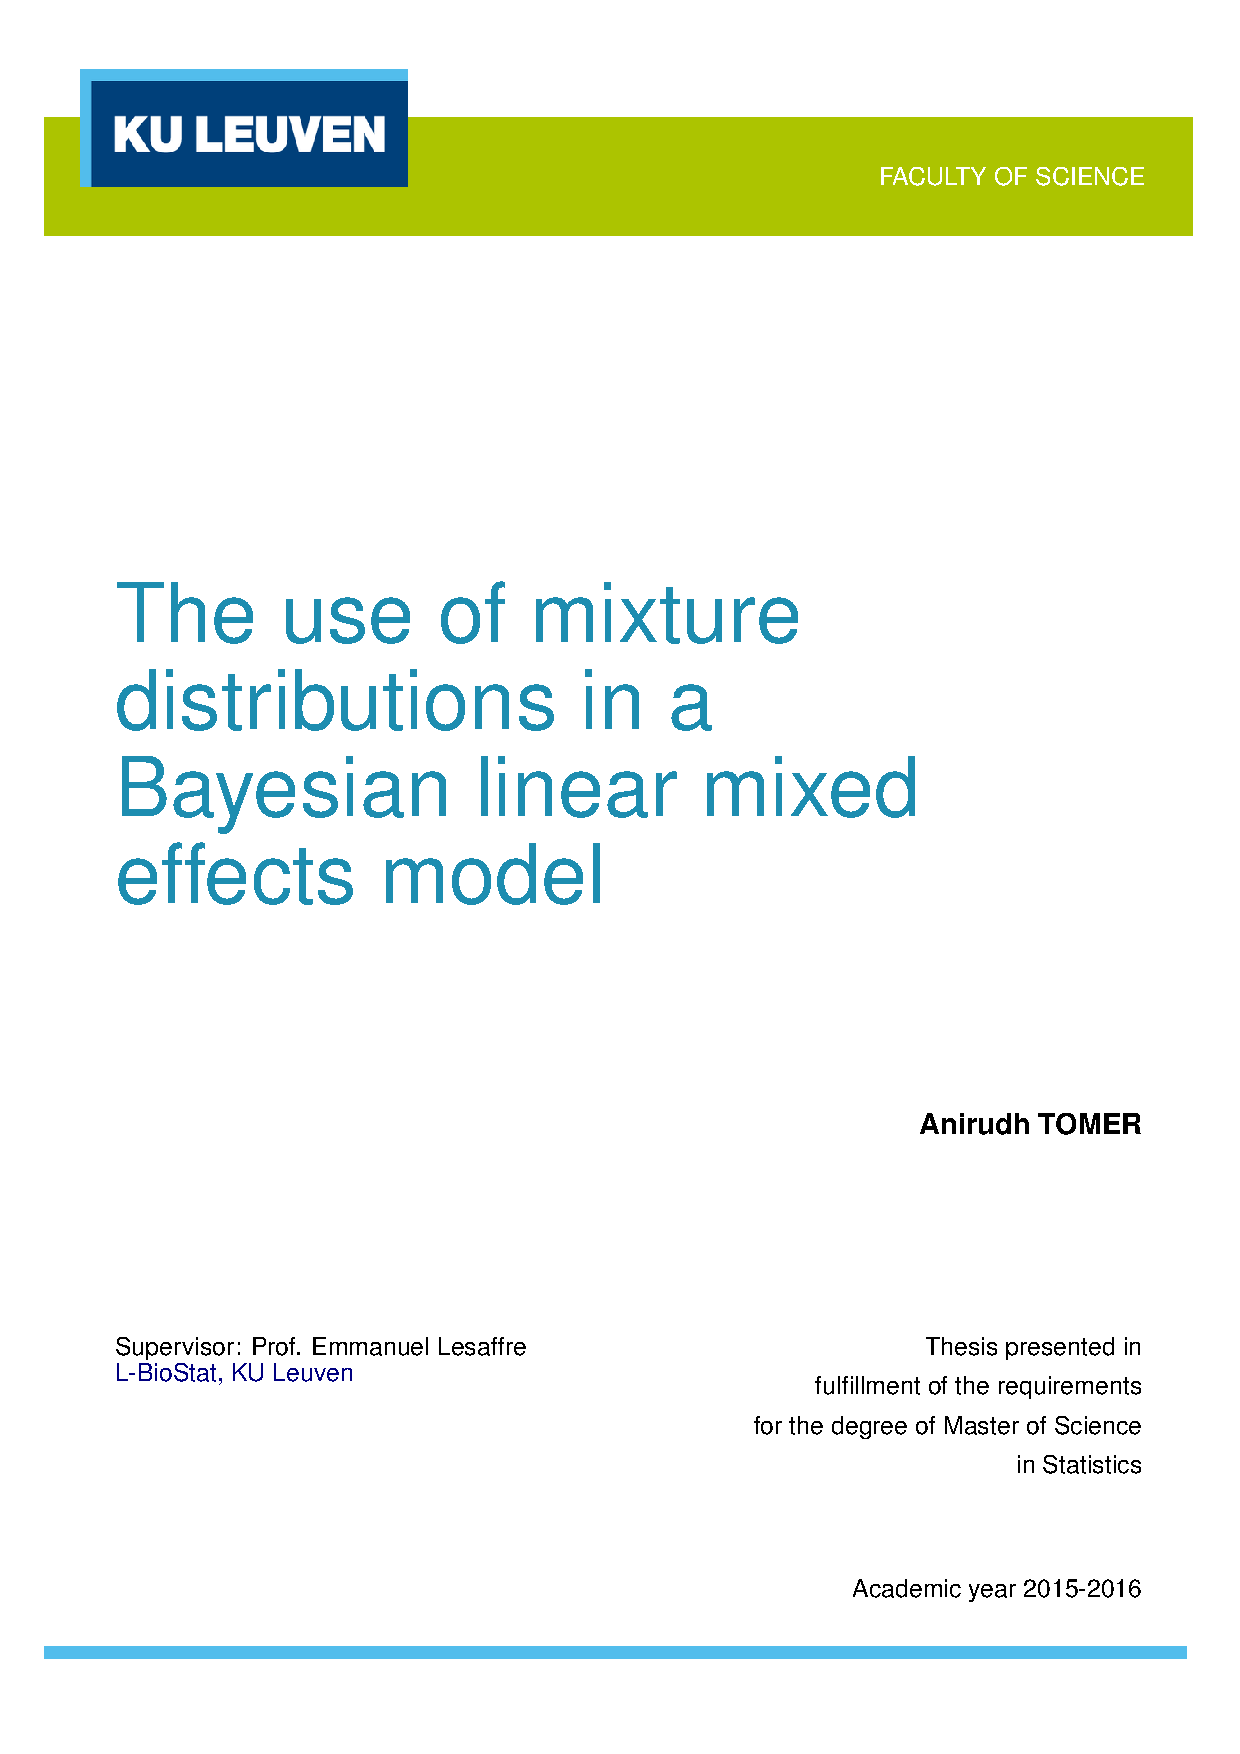
\includepdf[pages={1}]{coverpages/titlepage/titlepage.pdf}
%an empty page to make sure copyright gets printed on a new page
\clearpage \null \clearpage
\null
\vfill
\copyright~ Copyright by KU Leuven \\

Without written permission of the promotors and the authors it is forbidden to reproduce or adapt in any form or by any means any part of this publication. Requests for obtaining the right to reproduce or utilize parts of this publication should be addressed to KU Leuven, Faculteit Wetenschappen, Geel Huis, Kasteelpark Arenberg 11 bus 2100, 3001 Leuven (Heverlee), Telephone +32 16 32 14 01. \\

A written permission of the promotor is also required to use the methods, products, schematics and programs described in this work for industrial or commercial use, and for submitting this publication in scientific contests.
\cleardoublepage

% frontmatter + roman page numbers
\frontmatter

% !TEX root =  ../../thesis.tex

\chapter{Preface}
\label{ch : preface}

The following thesis work was conducted as part of the programme completion requirements of MSc. Statistics programme at KU Leuven. When I began working on this project, I had little idea that I would be able to go as far as I have been now. There were many significant obstacles on the way, such as analytical calculations of the various Deviance information criteria definitions, marginal likelihood, choice of posteerior predictive checks, implementating them in a software, Gibbs sampler idiosyncrasies and lack of computational power required for this work. However, at every step the work became more and more enticing. Looking backwards, I think it was one of the most interesting project I have done in recent times. Through and through, I enjoyed every bit of this project. The entire work for this thesis has been done using R and JAGS (Just Another Gibbs Sampler). The source code, results of simulations and an electronic draft of this thesis can be found at\\
\url{https://github.com/anirudhtomer/MScThesis}\\

In chapter 1 we present an introduction to mixture distribution and their central role in the formulation of the problem statement for this thesis. In Chapter 2 we present an introduction to the Bayesian paradigm as for the work of this thesis we use Bayesian methods. Futher in Chapter 3 we present the definition of a Bayesian heterogeneity model, and the issues with estimation of parameters in it. In Chapter 4 we present the formulae for various classes of Deviance information crieteria, marginal likelihood and posterior predictive checks that we used for model selection. Chapter 5 includes the results of the simulation study that was performed to check the efficacy of the aforemented Bayesian model selection methods. In chapter 6 we model the Blood donor data set \citep{nasserinejad_prevalence_2015} using a Bayesian heterogeneity model and use results from the simulation study to apply the right model selection criteria.\\

I am grateful to my supervisor Professor Dr. Emmanuel Lesaffre for keeping faith in my capabilities and for guiding me in the right direction. I enjoyed the fact that he never spoonfed me, yet was always available to discuss the difficult parts of the work at hand. He set very clear goals at the beginning of the year and continually monitored my progress thereafter. My interest in Bayesian statistics has grown by magnitudes under his supervision and I am looking forward to contribute more in this area. I would also like to extend my gratitude to Professor Geert Molenberghs and Professor Geert Verbeke for the captivating lectures on longitudinal data analysis. They introduced me to mixed models and empowered me with the tools of trade required to do the frequentist analysis of blood donor data set in this report. I am thankful to Kazem Nasserinejad from ErasmusMC for resolving many of my queries regarding the blood donor data set, and to Igor Milhoranca for providing the much needed inputs at crucial times. Lastly, I am grateful to my parents for the innumerable sacrifices they made to make sure I had as less obstacles as possible during my studies and I dedicate this work to them.\\

Anirudh Tomer\\
Leuven, Belgium\cleardoublepage
% !TEX root =  ../../thesis.tex

\chapter{Summary}
\label{ch : summary}

\todo[inline]{update the summary with the newest conclusions}

In this master thesis we fitted a finite mixture distribution for the random effects in a Bayesian linear mixed model. A mixture distribution for random effects allows to model the heterogeneity introduced by ignoring certain covariates in the mean structure of the model or to take into account the unknown non normal distriution for random effects. We then explored effectiveness of Bayesian model selection criteria (DIC, Bayes Factor, PPC) for choosing the number of component densities in the mixture distribution of random effects. Since mixture models are missing data models, we implemented various definitions of DIC as given by \citet{celeux_deviance_2006} for such models. We found that DIC 4 based on complete data likelihood was a fairly good selection criteria. However as the sample size decreased the discerning power of DIC also decreased. We then implemented Bayes Factor based on the approximation given by \citet{chib_marginal_1995} and found that it was not reliable for deciding on number of components required in the model. On the other hand, Posterior predictive checks were a very strong discerning method if indepdent inverse gamma priors were used for variance components, and uniform distribution for correlation, in the distribution of random effects. In regards to the choice of prior distribution for covariance parameters, we found that a Wishart prior for precision matrix(inverse of covariance matrix) overestimates the precision when within subject variance is greater than between subject variance. Thus, it could be a good idea to decrease scale of the intercept and the covariate corresponding to random slope, so that the corresponding variances increase in magnitude.
%\printglossary[type=\acronymtype,style=list,title={List of abbreviations}]
\cleardoublepage
\tableofcontents

% main matter (chapters + appendices
\mainmatter
% !TEX root =  ../../thesis.tex 

\chapter{Introduction}
\label{ch : introduction}

In this chapter we will first introduce the mixture distribution and then mention the challenges involved in estimation of parameters of a mixture distribution. We will also highlight the benefits of using a Bayesian approach for parameter estimation. Lastly we will present the goal of this master thesis, in which a mixture distribution plays the central role.

\section{Mixture distribution}
\label{sec : mixture_distribution}
A mixture distribution is a probability distribution of a random variable formed from a group of other random variables. The formation of a mixture distribution can be seen as a two step process, in which firstly a particular random variable is selected from a collection of random variables based on a certain probability of selection. In the second step a value is sampled for the selected random variable from its probability distribution. For e.g. the following random variable $Y$ has a mixture density formed from 3 normally distributed random variables.

$$Y \sim \dfrac{1}{6}N(-10,3) + \dfrac{1}{2}N(0,1) + \dfrac{1}{3}N(4,2)$$

\begin{figure}
	\centering
	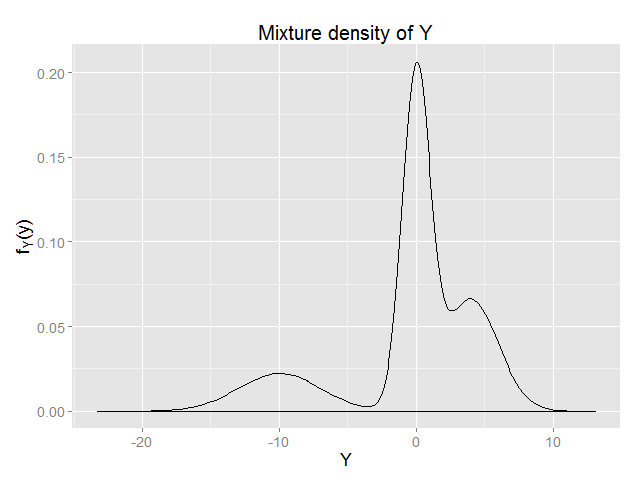
\includegraphics[scale=0.5]{mainmatter/chapter_1_introduction/mixture_density.png}
	\caption{Mixture density of $Y \sim \dfrac{1}{6}N(-10,3) + \dfrac{1}{2}N(0,1) + \dfrac{1}{3}N(4,2)$}
	\label{fig : mixture_density_1}
\end{figure}

Figure \ref{fig : mixture_density_1} shows the density function for $Y$. The density is trimodal with each mode corresponding to one of the components in the mixture. Mixtures like $Y$ which are formed from a finite sum of components are called finite mixtures. The components are also known as mixture components and their densities are called component densities. The constants multiplying the corresponding densities are called mixture weights. The mixture weights also represent the probability of selection of each component density. Each mixture weight should be positive and the sum of all mixture weights should be equal to 1. While in our example all the  mixture components were having the same parametric family i.e. Normal distribution, it is also possible to have mixture components from different parametric families. A mixture model where it is assumed that all data points are generated from a mixture of normally distributed component densities is called Gaussian mixture model (GMM). It is important to note that the idea of a mixture distribution is rather hypothetical, as in an example by \citet{titterington_statistical_1986} it was shown that a GMM of two components could be indistinguishable from a log-normal distribution.

\subsection{Formal definition for finite mixture distribution}
\label{subsec : formal_def_mixture_dist}
Given a finite set of $K$ probability density functions $p_1(y), p_2(y), \ldots, p_K(y)$ and weights $\eta_1, \eta_2, \ldots, \eta_K$, a random variable $Y$ is said to have a finite mixture distribution if

$$p(y) = \sum_{k=1}^{K} \eta_{k} p_{k}(y)$$

The vector of the weights $\boldsymbol{\eta} = (\eta_1, \eta_2, \ldots, \eta_K)^T$ is called the weight distribution. The $k^\text{th}$ weight $\eta_{k}$ corresponds to selection probability of the $k^\text{th}$ density while sampling for $Y$. It can only take values from the $K$ dimensional positive real coordinate space ${\mathbb{R}^{+}}^K$ with an additional constraint, $\sum_{k=1}^{K} \eta_{k} = 1$.\\

\subsection{Challenges}
\label{subsec : challenges_mixture_density}
The primary challenge while modeling a mixture density for a random variable is that the number of mixture components ($K$), weight distribution $\boldsymbol{\eta}$ and the corresponding parameters for component densities are rarely known in advance. Secondly, from a sample of $N$ observations $y_1, y_2, \ldots, y_N$ sampled from the mixture density $p(y)$ one may not know which observation belongs to which component density. Formally, an allocation vector $\boldsymbol{S} = (S_1, S_2, \ldots, S_N)^T$ represents the allocation of observations to mixture components. i.e. $S_i = k$ represents that $i^\text{th}$ observation belongs to $k^\text{th}$ component density. Estimating the allocation vector is in fact solving the clustering problem, albeit using parametric methods in our case.\\

While Maximum Likelihood based methods such as the EM algorithm could be used to deal with the above mentioned challenges, there are certain downsides to them. Firstly it is well known that 95\% confidence intervals of ML estimates are based on asymptotic normality of the estimators. Thus in case of small sample size, or small mixture weights the results will not be correct \citep[pg. 35]{fruhwirth-schnatter_finite_2013}. A Bayesian approach however is immune to these issues as the posterior distribution of parameters is allowed to be non-normal. Secondly, in case of univariate and multivariate GMM, the likelihood function

$$ p(\boldsymbol{y}|\boldsymbol{\mu}, \boldsymbol{\sigma^2}, \boldsymbol{\eta}) = \prod_{i=1}^{N} \sum_{k=1}^{K} f_N(y_i; \mu_k, \sigma^2_k) \eta_k$$

is unbounded and has many spurious nodes near the boundary of the parameter space for variance($\sigma^2_k$) of the components \citep{kiefer_consistency_1956,day_estimating_1969}. A Bayesian approach however, handles this problem elegantly using priors for parameters of the component densities. For e.g. \citet[pg. 176]{fruhwirth-schnatter_finite_2013} combined the likelihood with the prior $p(\mu_k, \sigma^2_k) \propto p(\sigma^2_k), \sigma^2_k\sim \text{Inv-Gamma}(1,4)$, and showed that it lead to a joint posterior density $p(\mu, \sigma^2 | \boldsymbol{y})$ of parameters in which $\sigma^2_k$ was bounded away from 0. Thus all the spurious nodes near the boundary of the parameter space for $\sigma^2_k$ were cut out, whereas they were apparent for the surface of the likelihood function.

\subsection{Applications of mixture distributions}
Mixture models have found usage in a variety of domains. Some of the examples are:
\begin{itemize}
\item Spike sorting of neural data: Both GMM and mixture of multivariate t-distributions have been used.\citep{lewicki_bayesian_1994,shoham_robust_2003}.
\item Speaker recognition as well as speech to text conversion algorithms have used mixture models \citep{simancas-acevedo_speaker_2001,xiang_efficient_2003,povey_subspace_2011}.
\item Image processing: GMM have been used to find features in an image, such as objects, boundaries etc. \citep{fu_color_2012}. For e.g. \citet{ming-hsuan_yang_gaussian_1998} have used GMM to model the distribution of skin color pixels. Many authors have also proposed using GMM for face recognition. i.e. as a biometric identification mechanism.
\item Finance: \citet{brigo_lognormal-mixture_2002} proposed to use a log-normal mixture distribution for pricing of financial assets.
\item Biology: Mixture models have found usage in genetics and cell biology.\citep{sim_evaluating_2012,gianola_mixture_2007} 
\end{itemize}

The example applications we cited involved usage of mixture models to adjust for a hidden attribute in the data which could not be collected or to approximate a density which is not of known form. However mixtures have also been used as supplementary methodology in various models, a list of which can be found in \citet[pg. 238]{fruhwirth-schnatter_finite_2013}. One such usage in linear mixed models has been proposed by \citet{verbeke_linear_1996} and it also forms the theme of this thesis.

\section{Goal of master thesis}
\label{sec : goal}
\citet*{verbeke_linear_1996} proposed to use a finite mixture distribution of normally distributed components for the prior distribution of random effects in a linear mixed effects model (LMM). This particular LMM is also known as Heterogeneity model. For the scope of this thesis our focus will be on the Bayesian version of the linear mixed effects model(BLMM), where all parameters involved are assigned a probability distribution. Needless to say, the issues described in section \ref{subsec : challenges_mixture_density} are also applicable for the Bayesian heterogeneity model. The aim of this master thesis is to evaluate existing Bayesian approaches for model selection, namely Deviance Information Criterion (DIC) , marginal likelihood and posterior predictive checks(PPC) for selecting the right number of mixture components for the distribution of random effects. Since we will be working in the Bayesian framework, we will use MCMC methods instead of the frequentist point estimation methods. We will simulate data sets to check efficacy of each of the aforementioned model selection criteria and then use the most effective ones to decide the number of mixture components for the random effects distribution in Blood donor longitudinal data set \citep{nasserinejad_prevalence_2015}.
% !TEX root =  ../../thesis.tex 

\chapter{Bayesian methodologies}
\label{ch:bayesian_methodologies}

\todo[inline]{Write something here}

\chapter{Mixture models}
\label{ch:mixture_models}

\todo[inline]{Write something here}

\chapter{Data set}
\label{ch:data_set}

\todo[inline]{Write something here}

\chapter{Analysis of data}
\label{ch:analysis_of_data}

\todo[inline]{Write something here}

\chapter{Conclusion}
\label{ch : conclusion}

\todo[inline]{Write something here}


% Appendices should go here
\appendix

% backmater => mainly references
\backmatter
\printbibliography
\cleardoublepage


\includepdf[pages={1}]{coverpages/backpage/backpage.pdf}
\end{document}
